\begin{lstlisting}
open util/integer

//--------MODEL:-------//

sig Name {}

sig Place {} 

sig Appointment {
place: one Place,
date: one Int,
time: Int,
duration: lone Int,
alert: lone Alert,
travel: one Travel
} {
date >0
time >0
duration>0
alert != none => alert.appointment = this 
travel.placeOfArrival = place
}

sig Alert {
appointment: one Appointment,
date: one Int,
time: one Int
} {
date >0
time >0
appointment.alert = this
}

sig Calendar {
appointments: set Appointment
}

sig User {
calendar: one Calendar,
email: one Name,
password: one Name
}

sig Movement {
placeOfDeparture: one Place,
placeOfArrival: one Place,
extimatedTime: one Int,
} {
placeOfDeparture != placeOfArrival
extimatedTime > 0
}

sig Travel {
placeOfDeparture: one Place,
placeOfArrival: one Place,
timeOfDeparture: one Int,
extimatedTime: one Int,
movements: some Movement,
} {
placeOfDeparture != placeOfArrival
extimatedTime > 0
timeOfDeparture > 0
}


//--------FACTS:-------//

//different users  have different email addresses
fact mailUnique {
no disjoint u1, u2: User | u1.email = u2.email
}

//different users have different calendars
fact calendarUnique {
no disjoint u1, u2: User | u1.calendar = u2.calendar
}

//different calendars have different appointments
fact appointmentsUnique {
all disjoint c1, c2 : Calendar | c1.appointments & c2.appointments = none
}

//a movement cannot exist outside of a travel
fact noMovementWithoutTravel {
Travel.movements = Movement
}

//a travel cannot exist without its appointment
fact noTravelWithoutAppointment {
Appointment.travel = Travel
}

//an appointment cannot exist outside of a calendar
fact noAppointmentWithoutCalendar {
Calendar.appointments = Appointment
}

//a calendar cannot exist without its user
fact noCalendarWithoutUser {
User.calendar = Calendar
}

//the alert of an appointment cannot be scheduled after the beginning 
//of the appointment
fact alertBeforeAppointment {
all a: Appointment | a.alert.date < a.date or (a.alert.date=a.date and 
	a.alert.time < a.time)
}

//every travel is composed by a sequence of connected movements
fact travelIsMadeByMovements {

//every travel starts with a movement
all t: Travel | (one m: t.movements | m.placeOfDeparture = t.placeOfDeparture)
//every travel ends with a movement
all t: Travel | (one m: t.movements | m.placeOfArrival = t.placeOfArrival)
//the ending of a movement is the beginning of a new one or 
//the end of the travel
all t: Travel | (all m: t.movements | m.placeOfArrival = t.placeOfArrival 
or
(one m1: t.movements | m1!=m and m.placeOfArrival = m1.placeOfDeparture))
//the beginning of a movement is the ending of an old one or the 
//beginning of the travel
all t: Travel | (all m: t.movements | m.placeOfDeparture = t.placeOfDeparture 
or
(one m1: t.movements | m1!=m and m.placeOfDeparture = m1.placeOfArrival ))
//different movements cannot start or end at the same position
all t: Travel | (no disjoint m1, m2: t.movements | m1.placeOfDeparture =
m2.placeOfDeparture
or
m1.placeOfArrival = m2.placeOfArrival )
//no close path
all t: Travel | (no m: t.movements | m.placeOfArrival = t.placeOfDeparture)

}

//the extimated time of a travel is the sum of the extimated times 
//of its movements
fact travelTimeSumOfMovementsTime {
all t: Travel | t.extimatedTime = sum (t.movements.extimatedTime)
}

//every traveal leads to the appointment in time
fact travelsInTime {
all a: Appointment | plus[a.travel.timeOfDeparture, a.travel.extimatedTime] 
= a.time													
}



//--------ASSERTIONS:-------//

//if a movement starts at the travel starting and ends at travel ending, 
//it's the only movement of the travel (and vice versa)
assert oneMovementTravel {
all t: Travel | all m : t.movements | m.placeOfDeparture = 
	t.placeOfDeparture and m.placeOfArrival = t.placeOfArrival <=> 
	t.movements = m
}	

//a movement nvere takes a longer time than the corresponding travel
assert noMovementLongerThanTravel {
all t:Travel | no m:t.movements | m.extimatedTime > t.extimatedTime
}



//--------PREDICATES:-------//
pred addAppointment [c1, c2: Calendar, a: Appointment] {
a not in c1.appointments implies c2.appointments = c1.appointments + a
}

pred deleteAppointment [c1, c2: Calendar, a: Appointment] {
c2.appointments = c1.appointments - a
}

pred addAlert [a1, a2: Appointment, al: Alert] {
a1.alert = none implies a2.alert = al
}

pred deleteAlert [a1, a2: Appointment, al: Alert] {
a1.alert = al implies a2.alert = none
}

pred show {}

check oneMovementTravel
check noMovementLongerThanTravel

run addAppointment
run deleteAppointment
run addAlert
run deleteAlert

run show for 3 but 8 Int, exactly 1 User, exactly 2 Travel, exactly 
3 Movement, exactly 1 Alert
run show for 3 but 8 Int, exactly 3 User, exactly 2 Appointment

\end{lstlisting}
\clearpage

\begin{figure}[!h]
	\centering
	\makebox[\textwidth][c]{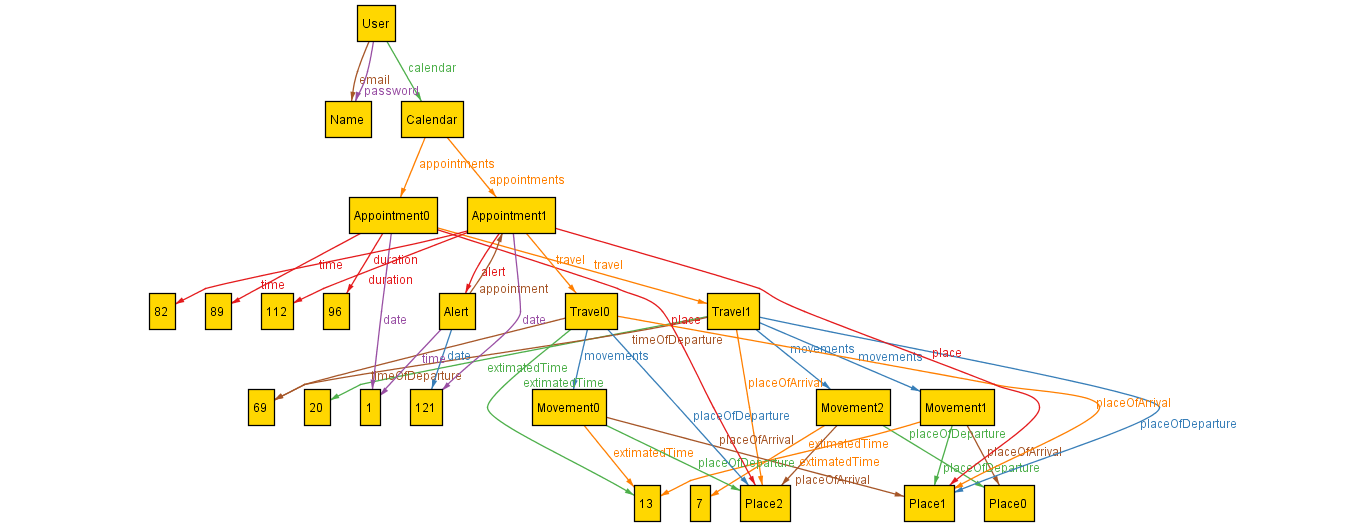
\includegraphics[width=1.3\textwidth]{Images/Alloy/World1.png}}%
	\caption{Alloy: first example}
\end{figure}

The first picture shows a world in which one user has more appointments in his calendar. Each appointment is associated with a travel:
\begin{itemize}
	\item Travel0: from Place2 to Place1 (location of Appointment1), extimatedTime = 13;
	\item Travel1: from Place1 to Place2 (location of Appointment0), extimatedTime = 20;
\end{itemize}

We notice that:
\begin{itemize}
	\item Travel0 = Movement0 (Place2 -> Place1, extimatedTime = 13);
	\item Travel1 = Movement1 (Place1 -> Place0, extimatedTime = 13) + Movement2 (Place0 -> Place2, extimatedTime = 7);
\end{itemize}

\begin{figure}[!h]
	\centering
	\makebox[\textwidth][c]{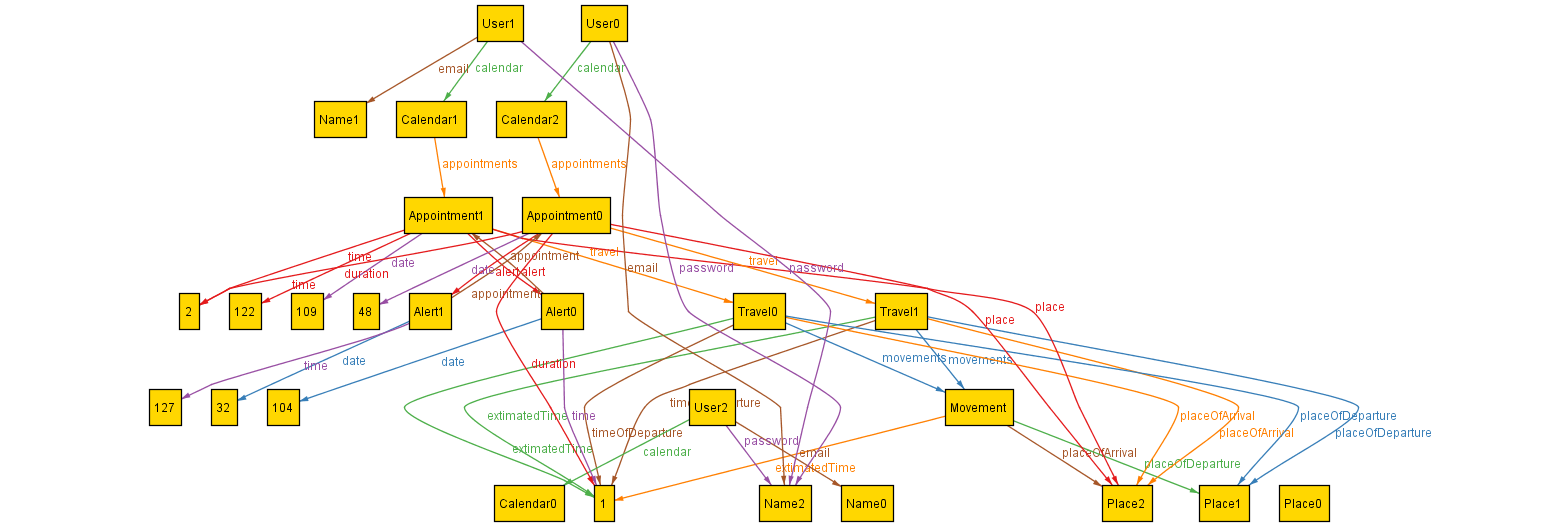
\includegraphics[width=1.3\textwidth]{Images/Alloy/World2.png}}%
	\caption{Alloy: second example}
\end{figure}
The second picture shows a world with more users.
